\section{Theoretical Background}

This chapter consists of all the background information needed to follow and understand what is included in this study. It gives an overall description on PWAs and React Native applications and their limits. How someone can evaluate usability, like usability testing is described, and an overall description of decision-making and the Multi-criteria Decision-making method Weighted Sum Method is presented. Finally, it talks about the work that has previously been done in the area.

\subsection{PWAs, React Native Applications, Native Applications and their differences}

A mobile application is a software application designed to run on a mobile device such as a smartphone. The two smartphone platforms which hold the majority of the market share at the time of writing are iOS and Android \cite{MarketShareGlobal2020}. 
Currently, three application development techniques are most commonly used \cite{ThreeAppTypes}:  Native, Web-based and Hybrid. 

Native applications are mobile applications developed to function on a specific platform. If a developer wants to release an application on several platforms, a native application has to be developed separately for each platform. 

Web-based applications utilise web servers to store data. This results in very low storage size on the user’s device but only allows for access when an internet connection is available. 

Hybrid applications are a mix between native and web-based applications. The idea is to write the majority of the code in a way that it can be compiled to run on several platforms. This is done by using a framework like Apache Cordova, Xamarin or React Native. Hybrid development allows for faster and more economic development than native development but produces applications which feel and function more native than web-based applications. 

\subsubsection{Progressive Web Application}

Progressive web applications (PWAs) work similarly as web-based applications, but by storing some data on the user’s device they can be accessed offline \cite{AppsWhatsTheDifference}.  PWAs can also access more hardware and functions than web-based applications. PWAs are typically not downloaded through the platforms own application distribution service, but rather accessed through the web browser of the device. 
Accessing the device hardware through the web browser adds another level of abstraction. This means a PWA is not able to access hardware to the same extent as native applications. 

The functionality of PWAs is significantly better on Android devices than on iOS devices \cite{AppsWhatsTheDifference}. The term PWAs was originally coined by Google in 2015  \cite{PWABook2019}, and Safari did not have support for the technology until 2018  \cite{PWAiOS,iOS113}. Some functionalities are still, at the time of writing, unavailable on iOS devices. A few of these features can be found in table \ref{tab:yes-no-features}.

\begin{table}[ht]
    \centering
    \begin{tabular}{ |c|c|c|c|c|c| } 
        \hline
        \rowcolor{light-gray}
        Feature & Android & iOS & Feature & Android & iOS\\
        \hline
        Screen orientation \& lock & Yes & No & Bluetooth & Yes & No \\ 
        \hline
        Credentials & Yes & No & Push messages & Yes & No \\ 
        \hline
        Background sync & Yes & No & Local notifications & Yes & No \\ 
        \hline
        Advanced Camera Control & Yes & No & VR and AR & Yes & No \\
        \hline
        Vibration & Yes & No & Recording media & Yes & No\\
        \hline
    \end{tabular}
    \caption{\label{tab:yes-no-features}Selection of functions that work on Android but not on iOS for PWA.}
\end{table}

Some functions remain unavailable on both platforms. The lack of advanced sensors and contact information are two major limitations, inhibiting some uses for PWAs. The lack of NFC support, for example, makes contact-less payments impossible. Some functions have been experimented with, but have not appeared as officially available. A selection of these features can be found in table \ref{tab:no-feature}.

\begin{table}[ht]
    \centering
    \begin{tabular}{ |c|c|c|c|c|c| } 
        \hline
        \rowcolor{light-gray}
        Feature & Android & iOS & Feature & Android & iOS\\
        \hline
        Proximity sensors & No & No & Contacts & No & No \\ 
        \hline
        Geofencing & No & No & NFC & No & No \\ 
        \hline
        Task scheduling & No & No & Ambient light & No & No \\ 
        \hline
    \end{tabular}
    \caption{\label{tab:no-feature}Selection of features that do not work on either iOS or Android for PWA.}
\end{table}

\subsubsection{React Native}

React Native developed applications have access to more functions than PWAs. A drawback of using React Native is the poor performance aspect. Due to its single-threaded nature, JavaScript is not optimal for heavy computing, therefore applications heavy in graphics tend to perform poorly when developed as React Native applications or PWAs compared to native applications \cite{JSmultithread}.

When developing a React Native application, a frame is first built. Then, for each platform, this frame is built upon to make the application act like a platform-native application. About 95\% of the code is commonly built as cross-platform, and the remaining is platform-specific \cite{Ganguly2018}, but this number can vary depending on the application. This means developing a React Native application is more budget-friendly than developing two or more native applications. However, the development of React Native applications demands knowledge of the different platforms. This differs from a PWA, where knowing JavaScript is enough to develop one cross-platform application.

\subsection{Evaluating usability}

Performing usability tests is a resource-efficient way of testing a product's usability, as not so many tests are required to find a majority of issues. After just 15 tests, as much as 90\% of problems with the product can normally be found \cite{SixMacefield2016}.

There are several ways to test a solution’s usability \cite{MartinBella2012Umod}. One could for example conduct Remote Moderated Research, where the test subjects use the application during their own time and then report back to the researcher how they feel about the product they have tested. This method is useful when it is vital to the test that the product is tested during a specific time or activity, in a specific place or for a longer time period \cite[p.~353]{MartinBella2012Umod}. With this method, there is however a delay in receiving feedback from the test subjects. 

There is also the option of A/B testing where the test subjects, in a controlled environment, get to test out two (or more) versions of the same product. After the tests, the subjects rate the solutions and communicate their preference. This method is good for choosing between two alternatives. This could, for example, be two different graphical elements, or two different wordings. A/B testing most useful when a choice of product has to be made, but it does not answer the question of why the subject chose a certain solution. \cite[p.~12]{MartinBella2012Umod}. 

Group discussions, such as focus groups, are also an option for usability testing. Several subjects get to sit together and review the products. When there are plenty of test subjects to utilize, this is an efficient way to get several people’s opinions at the same time. However, for a first-hand experience test, it demands that there are enough devices to test on and resources to capture all participants’ thoughts and feelings about the product. \cite[p.~228]{MartinBella2012Umod}. 

Comparative usability testing is another alternative for conducting a usability test. A subject gets to test two (or more) products in front of the researcher, and the researcher notes the subject’s reactions to the products. This method is resource-efficient and only demands one device to test on. It is also relatively robust, as the tests are performed separately on different subjects, small errors will not affect the outcome of the study as a whole \cite{Ross2017}. The test subjects would test both applications, to maximize the input from the subjects on each version.

\subsubsection{Conducting a Usability test}

In order to conduct a usability test, one needs to design a number of tasks or scenarios for the test subjects to perform. The subject will perform these tasks under the supervision of the moderator \cite{Brooke2018}. The moderator is there to introduce the applications and to help the subject to proceed if they get stuck. A person, referred to as a recorder, takes notes from the test. This is useful since the moderator might be too busy with the test subject to properly record what is happening. 
Test subjects are encouraged to think out loud, giving the researchers qualitative data in real-time. This also allows the moderator to ask questions during the test, to further understand how the test subject's reactions to the product. 
The tests are documented, using a camera angled at the device being tested and/or a camera aimed at the participants’ face. This is done to conserve the qualitative data, allowing for later analysis. The setup for the tests looks like the example in figure \ref{fig:usability-test-example}.

\begin{figure}[ht]
    \centering 
    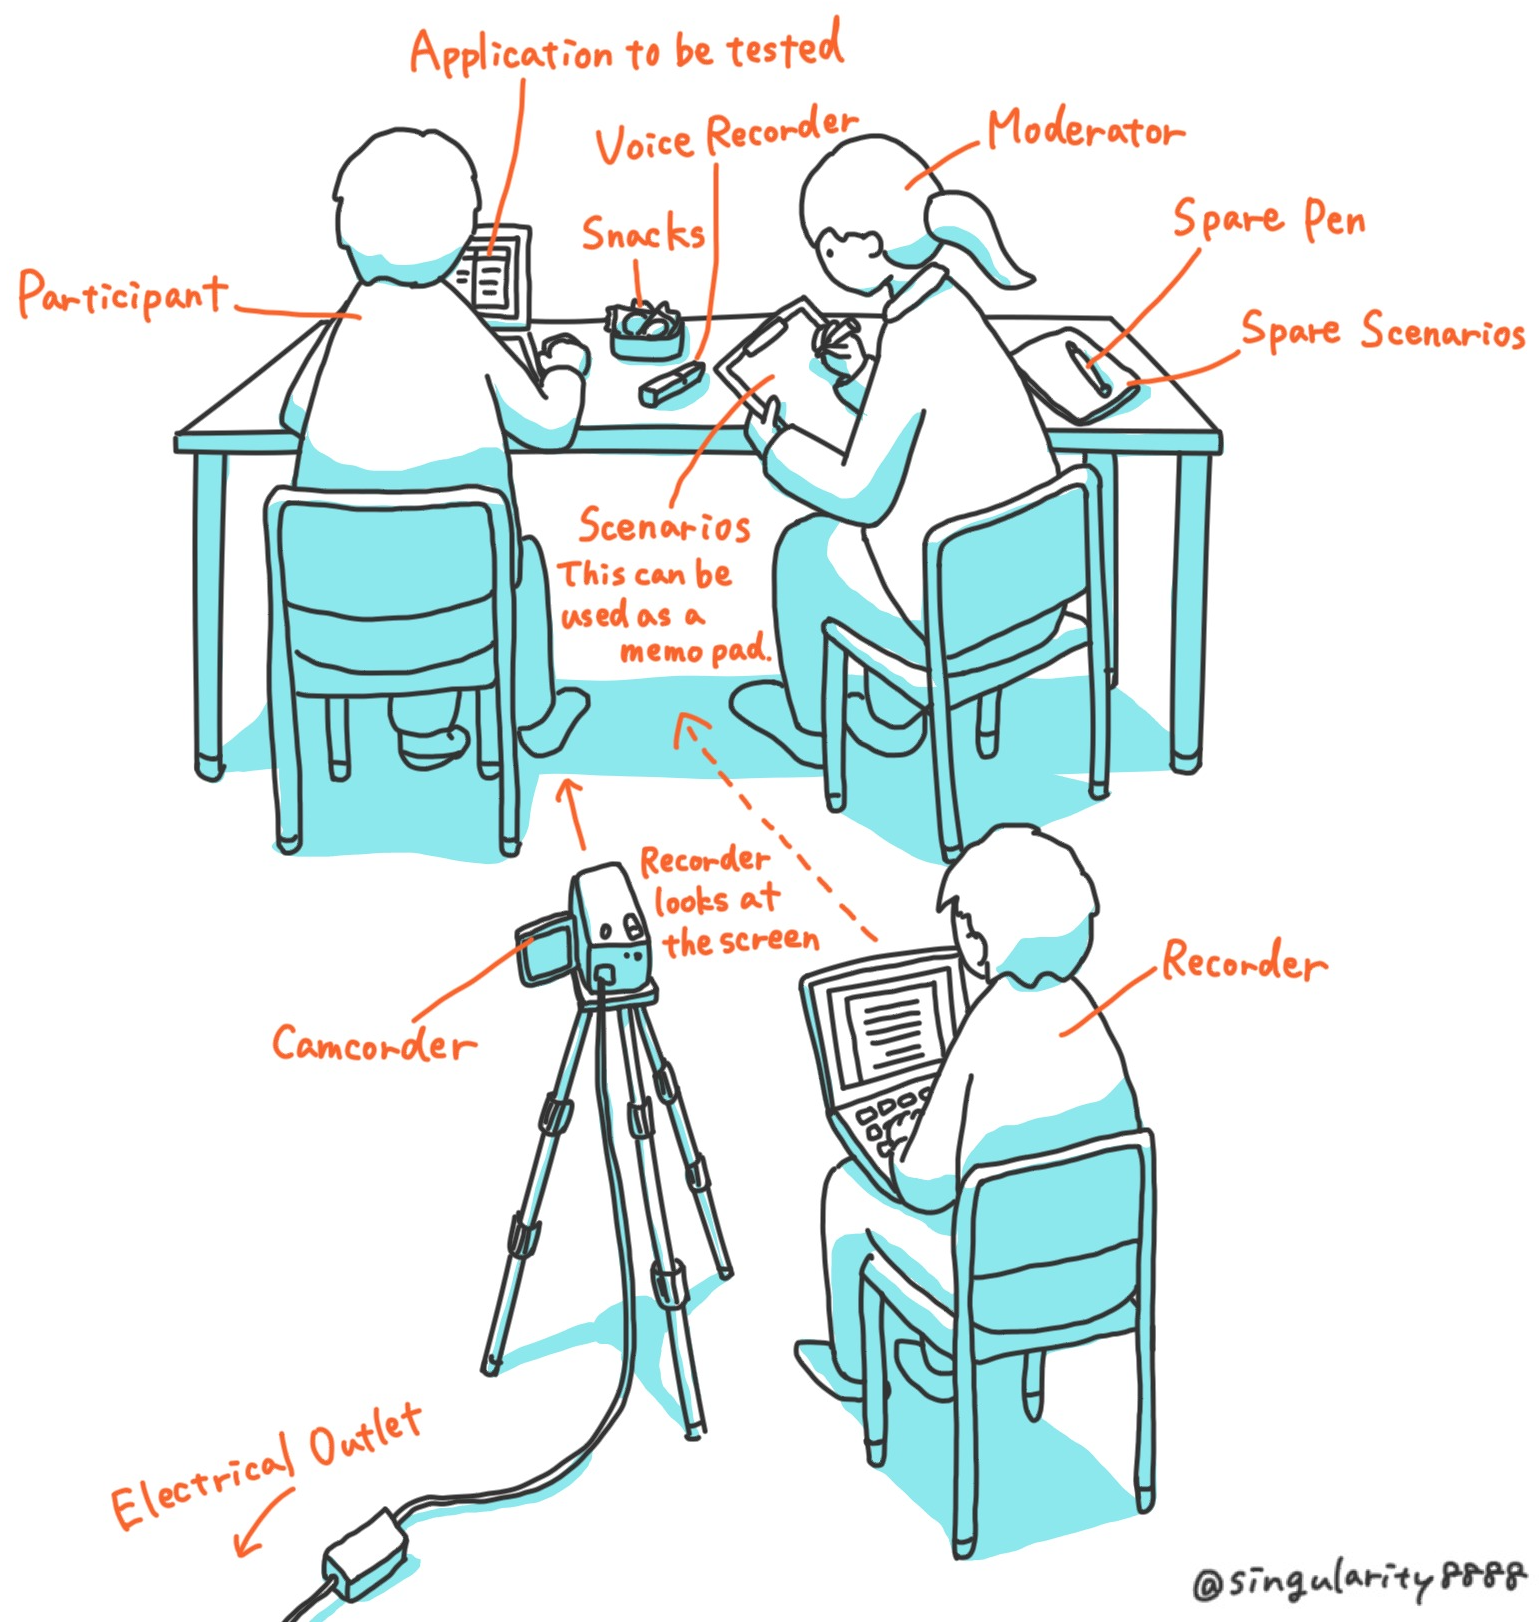
\includegraphics[width=0.75\textwidth]{img/usability_test_example.png}
    \hfill
    \caption{\textit{Diagram of conducting a simple usability test \cite{Shingyouchi2019}.  }}
    \label{fig:usability-test-example}
\end{figure}

To collect quantitative data efficiently, one can utilize forms and questionnaires in their usability tests. The subject assesses the products after, or during, the tests. 
The System Usability Scale (SUS) is an easy technique that is reliable even on small sample sizes \cite{SUSUsability}. It uses 10 items that can each be rated on 5 steps from Strongly agree to Strongly disagree, shown in figure \ref{fig:sus-questions-example}. 

\begin{figure}[ht] 
    \centering 
    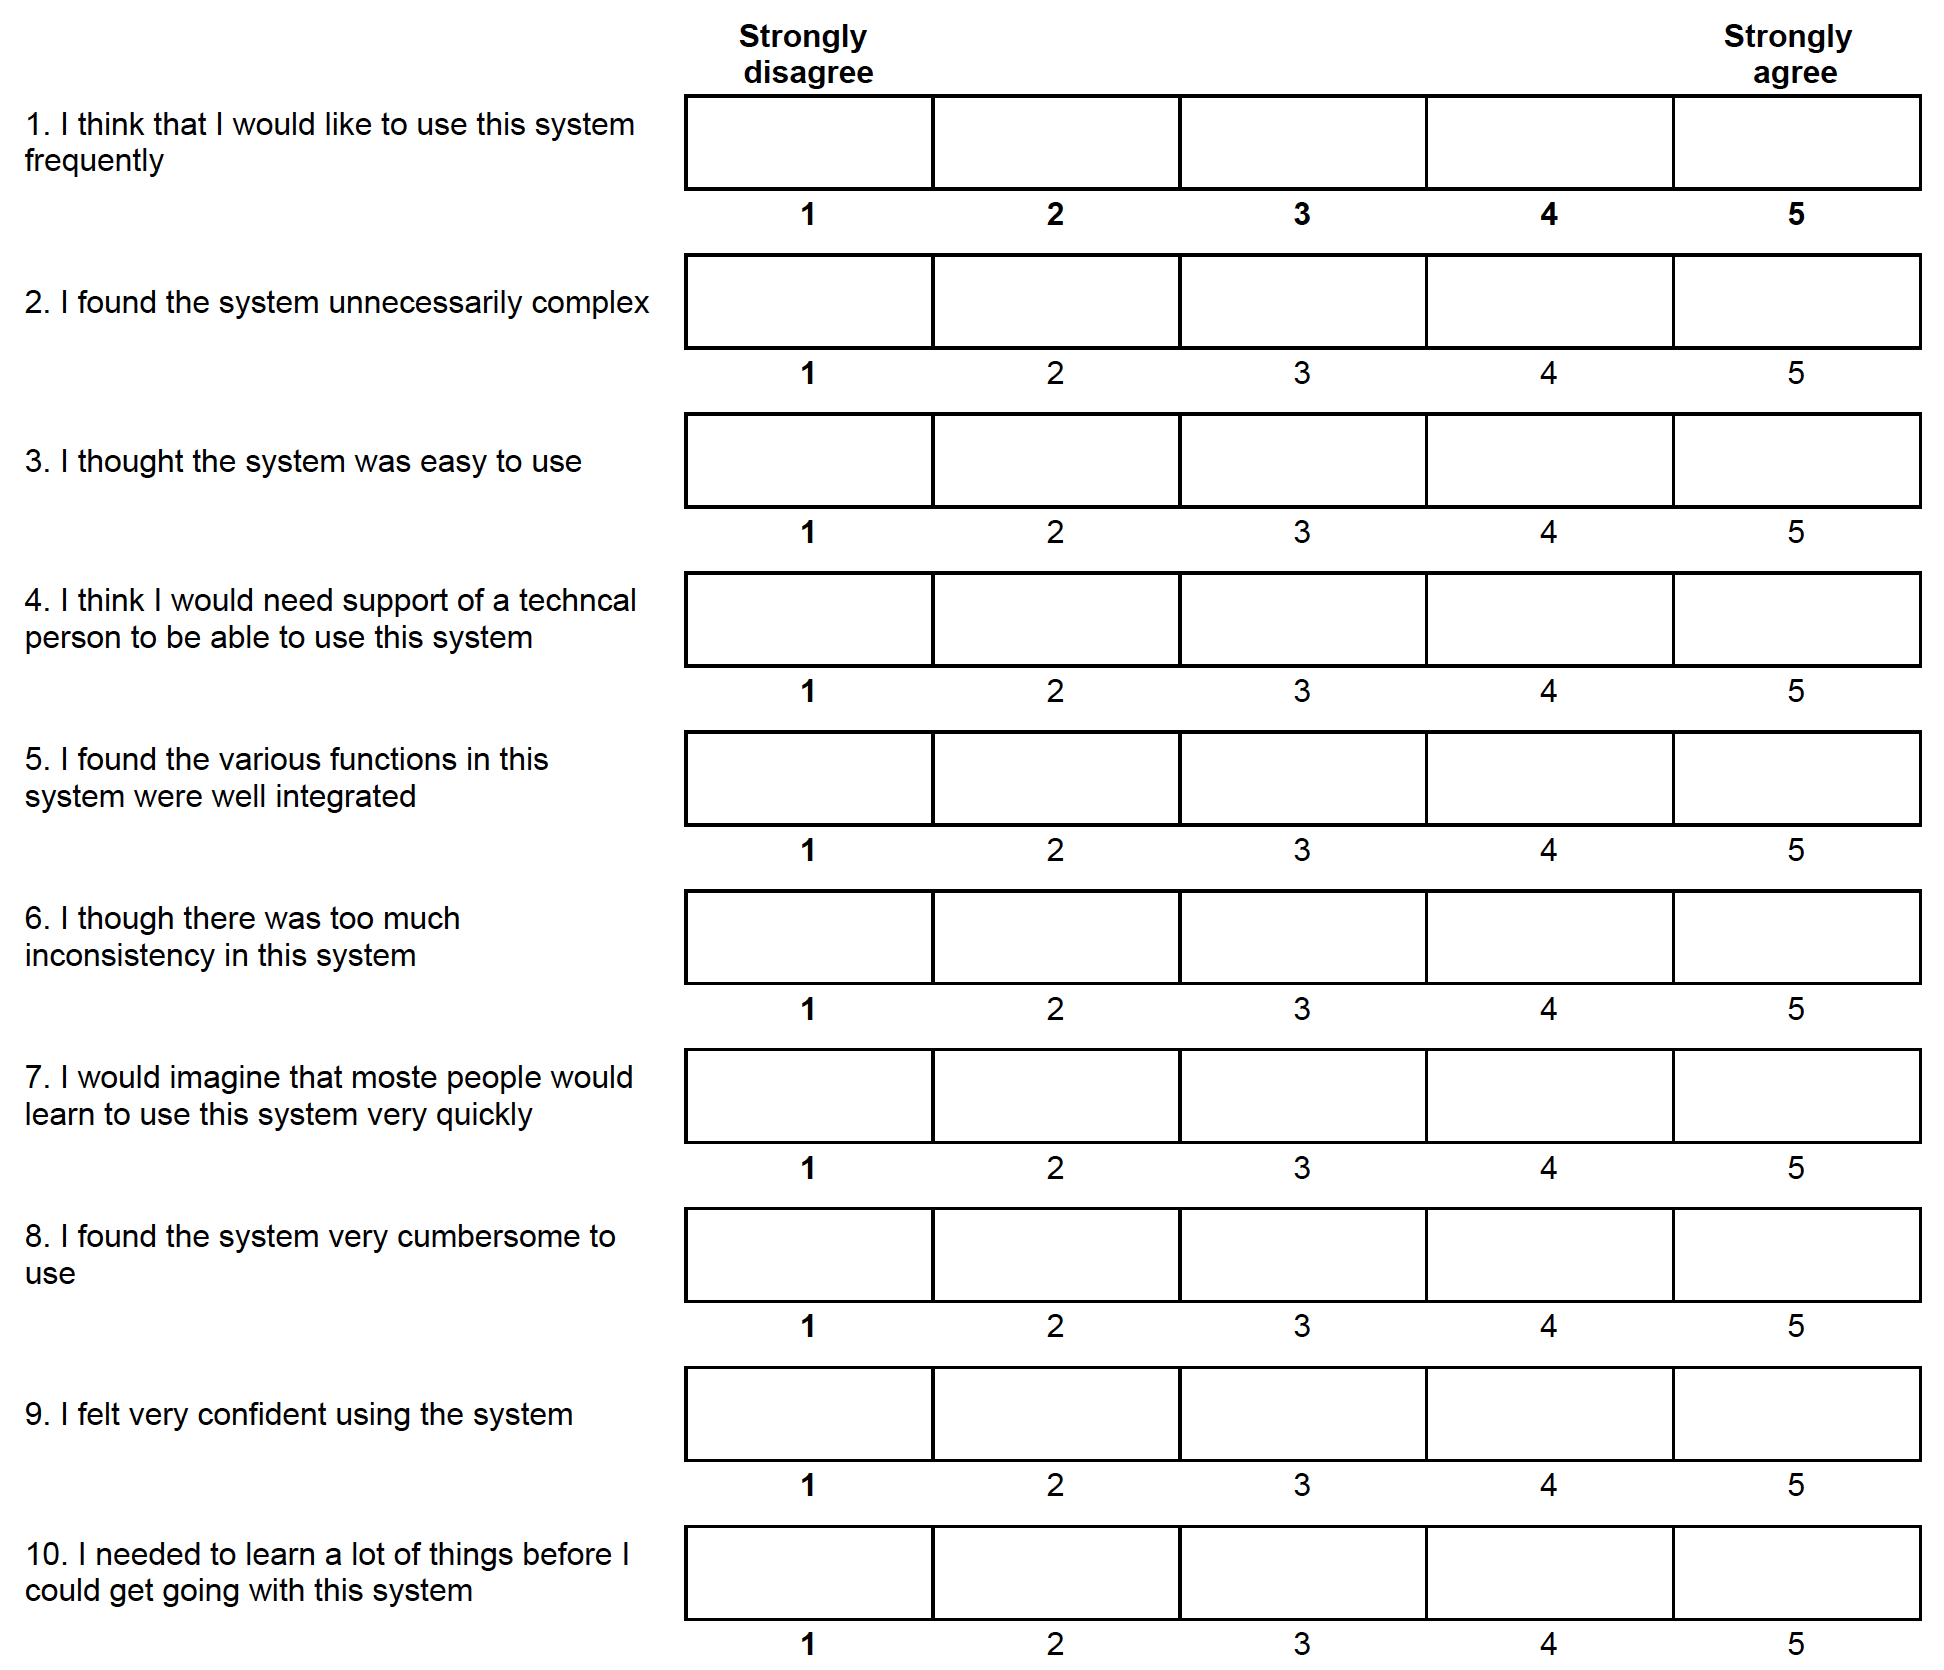
\includegraphics[width=0.8\textwidth]{img/sus_questions_example.png}
    \hfill
    \caption{\textit{SUS questions \cite{SUSUsability}.}}
    \label{fig:sus-questions-example}
\end{figure}

Calculating the SUS Score is done by doing the following; for every odd-numbered question, subtract 1 from the score. For every even-numbered question, subtract the score from 5. Sum the scores from all questions, then multiply the total with 2.5. The score will then get a grading that is based on known results shown in table \ref{tab:sus-grading}.

\begin{table}[ht]
    \centering
    \begin{tabular}{ |c|c|c| } 
        \hline
        \rowcolor{light-gray}
        SUS Score & Grade & Adjective Rating\\
        \hline
        >80.3 & A & Excellent \\ 
        \hline
        68 - 80.3 & B & Good \\ 
        \hline
        68 & C & Okay \\ 
        \hline
        51 - 68 & D & Poor \\
        \hline
        >51 & F & Awful \\
        \hline
    \end{tabular}
    \caption{\label{tab:sus-grading}Grading system for SUS.}
\end{table}

The user experience questionnaire (UEQ) seen in figure \ref{fig:UEQExample} is a fast and reliable way to measure both usability aspects and user experience aspects \cite{UEQOnline}. 
The UEQ can be separated into 6 categories: Attractiveness, Perspicuity, Efficiency, Dependability, Stimulation and Novelty. 
All questions in the questionnaire affect the score of one of these categories. 
If the result from one of the categories is not needed for the test, it’s corresponding questions can be left out of the questionnaire. A UEQ comparing two different versions of a product could produce a result as shown in figure \ref{fig:UEQExampleResult}. 

\begin{figure}[ht]
    \centering 
    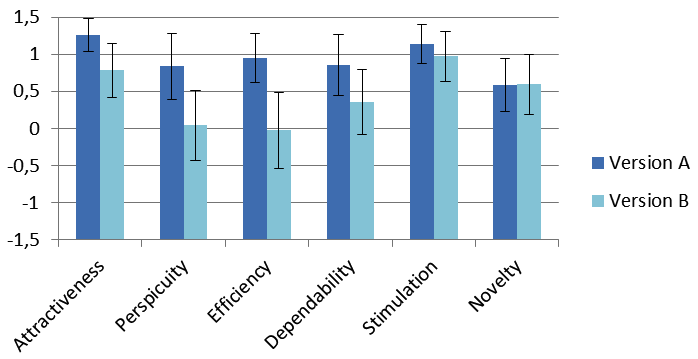
\includegraphics[width=0.9\textwidth]{img/comparative_test_ueq.png}
    \hfill
    \caption{\textit{UEQ result of a comparison between two versions of a product. The mean of each product on each category presented in blue bars, the confidence interval marked in black \cite{SchreppHinderksYhomaschewski2014}. }}
    \label{fig:UEQExampleResult}
\end{figure}

\begin{figure}[ht] 
    \centering 
    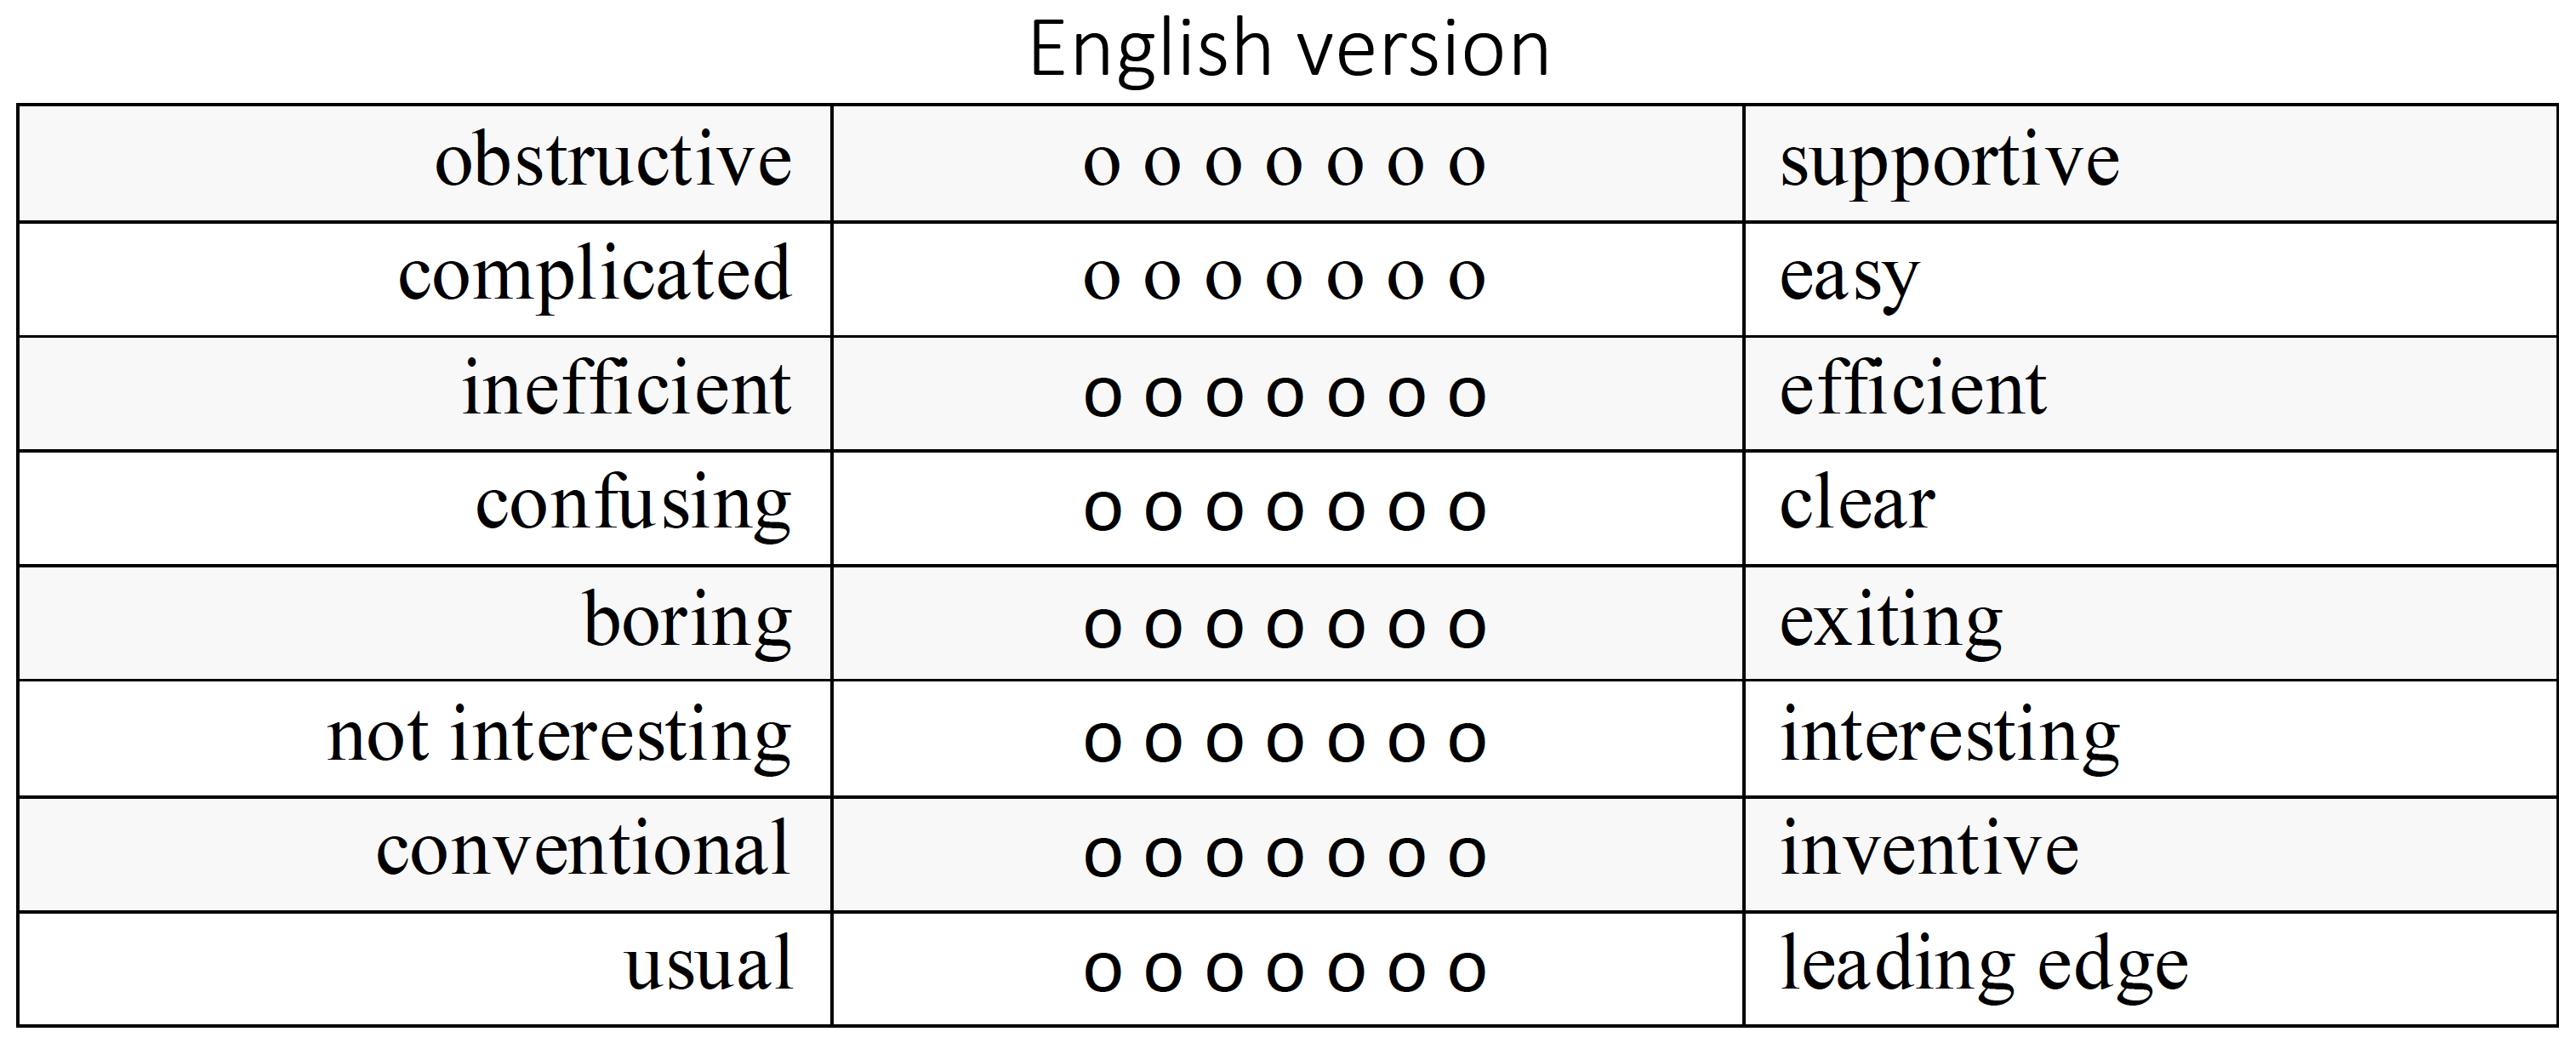
\includegraphics[width=0.9\textwidth]{img/ueq_questions_example.png}
    \hfill
    \caption{\textit{ Example of UEQ questions \cite{UEQOnline}. }}
    \label{fig:UEQExample}
\end{figure}

\newpage


\subsection{Decision making}

Decision-making is the practice of choosing an alternative based on available information. 
When the decision is based on many criteria, the process of choosing the optimal alternative falls under Multiple-criteria decision making.

\subsubsection{Multiple-criteria decision making}
Multiple-criteria decision making (MCDM), a collective term for different ways to optimally choose an alternative of something based on multiple, possibly conflicting, criteria \cite{MCDA}. 
The criteria of an MCDM can be factors such as cost, convenience, quality etc. In most decisions, the criteria have varying importance. 
This is represented by giving the criteria different weight, such that a criterion with high weight is more crucial to the final decision than one with a low weight. 

 A very common method for the MCDM is the Weighted Sum Model (WSM)  \cite[p.~6]{TriantaphyllouEvangelos2000MDMM}. With WSM, all criteria are given weight by the decision-maker, and each alternative is given a score on each criterion. For each alternative available, the weight of every criterion is multiplied by the score. These numbers are summed, producing a WSM-score for each alternative. The alternative with the highest WSM-score is the optimal solution. The WSM uses relatively simple mathematics, but it requires the data in the model to be quantifiable.  
 
Another popular method is the Analytical Hierarchy Process \cite{Vargas2010}, which works by doing a pair-wise comparison of each criterion. One flaw with this method is that it’s not very good at dealing with many criteria, as the decision-maker has to remember what they decided on previous comparisons and why, or else they risk making contradictory rankings  \cite[p.~11]{TriantaphyllouEvangelos2000MDMM}.

\subsubsection{Weighted Sum Method Example}

An example of a WSM: Charlie is choosing a car. They have three alternatives to choose between: A Kia Picanto, an Audi A8 and a Rolls Royce Phantom. 
Charlie has the following criteria to take into consideration: Price, Comfort, Performance and Prestige. The weights for each criterion and the score for each alternative is shown in table \ref{tab:WSM-Example}.

\begin{table}[ht]
    \centering
    \begin{tabular}{ |c|c|c|c|c| } 
        \hline
        \rowcolor{light-gray}
        & Price & Comfort & Performance & Prestige\\
        \hline
        \cellcolor{light-gray}Weight & 0.50 & 0.25 & 0.20 & 0.05 \\ 
        \hline
        Kia Picanto & 10 & 3 & 2 & 1 \\ 
        \hline
        Audi A8 & 6 & 6 & 8 & 5 \\ 
        \hline
        Rolls Royce Phantom & 1 & 10 & 10 & 10 \\
        \hline
    \end{tabular}
    \caption{\label{tab:WSM-Example}Weighted sum model matrix example.}
\end{table}

The weights indicate how important the different criteria are to the decision-maker. Charlie has set the highest score on the criterion Price, meaning they think that Price is the most important criterion.

The score for each criterion shows how well an alternative fulfils a criterion. A higher score indicates that the alternative is more superior in a criterion, for example, the Rolls Royce Phantom has a score of 10 on Comfort, indicating that it is a very comfortable car compared to the other alternatives.

Formula (\ref{eq:WSM-formula}) is used to calculate the WSM-score. \textit{a} refers to the alternatives, \textit{n} is the number of criteria, \textit{m} is the number of alternatives and \textit{w} is the score of each alternative on a criterion.

\begingroup
    \Large
    \begin{equation} \label{eq:WSM-formula}
        A_i^{WSM-score}=\sum_{j=1}^{n} \ w_j a_{ij}, \ for \  i = 1, 2, 3, ... , m
    \end{equation}
\endgroup

\begin{table}[ht]
    \centering
    \begin{tabular}{ |c|c| } 
        \hline
        \rowcolor{light-gray}
        Car model & WSM-score \\
        \hline
        Kia Picanto & 6.2 \\
        \hline
        Audi A8 & 6.35 \\
        \hline
        Rolls Royce Phantom & 5.5 \\
        \hline
    \end{tabular}
    \caption{Example WSM score for the example in table \ref{tab:WSM-Example}}
    \label{tab:WSM-score}
\end{table}

As seen in table \ref{tab:WSM-score}, in this scenario, the most favourable option for Charlie would have been the Audi A8, with the Kia Picanto coming in as a close second.

\subsection{Related Work}

Comparisons between web applications and native applications have been performed before \cite{Randleff2019}. This study, however, did not take PWAs or hybrid solutions into account. This study also did not take other factors apart from responsiveness into account when measuring the user experience.

PWAs have been compared to native applications in a study by Viktor Yberg \cite{Yberg2018}. This study compares the performance aspect of the two techniques and also explored the UX differences. However, this study's UX assumptions were based on a study \cite{Jobe2013} performed on native applications versus web applications, not PWAs.

Hardware responsiveness of PWAs has been tested in one study \cite{Fransson2017}. This study focused on Android and only researched the response time of the camera and GPS of a device. Another study \cite{HansenGronli2017} compared performance in launch-time, installation size and rendition time consumption.

A study has been made on the usability of Web applications and Hybrid applications \cite{KoziokasPanagiotisTselikas2017}, but did not include PWAs.

The usability of PWAs versus native applications has been investigated in a study comparing web applications, native applications and PWAs \cite{AndradeMartinez2018}. This study only performed a qualitative study on an Android device.
